\documentclass[a4paper]{article}

\usepackage[toc,page]{appendix}

\usepackage[spanish]{babel}
\usepackage[utf8]{inputenc}
\usepackage{amsmath}
\usepackage{graphicx}
\usepackage{fancyhdr}
\usepackage{amsmath}
\usepackage[colorinlistoftodos]{todonotes}
\usepackage{xcolor}
\usepackage{minted}
\usepackage[font=small,labelfont=bf]{caption}
\usepackage{enumitem}
\usepackage{textcomp}
\usepackage{siunitx}
\usepackage{textgreek}
\usepackage{bigints}
\usepackage{amsfonts}

\usepackage{hyperref}

\hypersetup{
    colorlinks,
    citecolor=blue,
    filecolor=blue,
    linkcolor=blue,
    urlcolor=blue
}

\usepackage{geometry}
\geometry{a4paper}

\begin{document}
\begin{figure}
\centering

\includegraphics[scale=1]{./img/logo}
\end{figure}

\title{\large\textsc{EAMTA 2019 - Advanced Digital Design}}

\author{
Andrew Parlane \\
}

\maketitle

\newpage

\section{Objetivo}

El objetivo de este curso estuvo implementar un micro básico en verilog, sintesizarle y hacer place and route, para generar las mascaras necesarios para fabricarle.

\section{Micro en Verilog}

El diseño del MICRO consiste en 5 módulos: Mux4, RegBank, ALU, Control y Top. Elige implementar todos con systemverilog. Todo el código es disponible en mi \href{https://github.com/andrewparlane/EAMTA2019}{GitHUB}.

Escribe testbenches bastantes completos para todos (excepto del Top) los módulos también usando systemverilog assertions. Usandos estos testbenches encontré varios errores y les arreglé. Por ejemplo al principio mi ALU estuvo equivocando unas operaciones, tuve que marcar las entradas y la salida como ``signed''.

Para compilar y ejecutar las simulaciones con VCS / SIMV ejecuto los siguientes commandos:

\begin{verbatim}
vcs -debug -sverilog -assert enable_diag ../../rtl/pkg/*.sv \
        ../../tb/OneBitAdder_tb.sv ../../rtl/*.sv
./simv -assert verbose -assert report +define+ASSERT_ON
vcs -debug -sverilog -assert enable_diag ../../rtl/pkg/*.sv \
        ../../tb/Mux4_tb.sv ../../rtl/*.sv
./simv -assert verbose -assert report +define+ASSERT_ON
vcs -debug -sverilog -assert enable_diag ../../rtl/pkg/*.sv 
        ../../tb/RegisterBank_tb.sv ../../rtl/*.sv
./simv -assert verbose -assert report +define+ASSERT_ON
vcs -debug -sverilog -assert enable_diag ../../rtl/pkg/*.sv \
        ../../tb/ALU_tb.sv ../../rtl/*.sv
./simv -assert verbose -assert report +define+ASSERT_ON
\end{verbatim}

Los sencillos (Mux4 y RegisterBank) funcionaron bien dando lo siguiente

\begin{verbatim}
    Chronologic VCS simulator copyright 1991-2017
Contains Synopsys proprietary information.
Compiler version M-2017.03-SP2-11_Full64;
Runtime version M-2017.03-SP2-11_Full64;
Mar 14 13:37 2019
Summary: 1 assertions, 0 with attempts, 0 with failures
           V C S   S i m u l a t i o n   R e p o r t 
Time: 4000 ns
CPU Time:      0.200 seconds;       Data structure size:   0.0Mb
Thu Mar 14 13:37:52 2019

    Chronologic VCS simulator copyright 1991-2017
Contains Synopsys proprietary information.
Compiler version M-2017.03-SP2-11_Full64;
Runtime version M-2017.03-SP2-11_Full64;
Mar 14 13:38 2019
$stop at time 460 Scope: RegisterBank_tb File: ../../tb/RegisterBank_tb.sv Line: 71
ucli% q
Summary: 6 assertions, 0 with attempts, 0 with failures
           V C S   S i m u l a t i o n   R e p o r t 
Time: 460 ns
CPU Time:      0.230 seconds;       Data structure size:   0.0Mb
Thu Mar 14 13:38:37 2019
\end{verbatim}

Tuve unos problemas con mis assertions en los testbenches más complicados y no tuve tiempo depurarles, pero funcionaron bien en modelsim dando me lo siguiente:

\begin{verbatim}
# ---------------------------------------------------------------------
# Name                          File(Line)                 Failure Pass
#                                                                                                              Count   Count
# ---------------------------------------------------------------------
# /OneBitAdder_tb/.../immed__21 OneBitAdder_tb.sv(21)       0     8

# ------------------------------------------------------------------------
# Name                           File(Line)                   Failure Pass
#                                                                                                                                                  Count   Count
# ------------------------------------------------------------------------
# /RegisterBank_tb/.../immed__42 RegisterBank_tb.sv(42)       0     1
# /RegisterBank_tb/.../immed__48 RegisterBank_tb.sv(48)       0     1
# /RegisterBank_tb/.../immed__54 RegisterBank_tb.sv(54)       0     1
# /RegisterBank_tb/.../immed__60 RegisterBank_tb.sv(60)       0     1
# /RegisterBank_tb/.../immed__66 RegisterBank_tb.sv(66)       0     1
# /RegisterBank_tb/.../immed__69 RegisterBank_tb.sv(69)       0     1

# ---------------------------------------------------------------
# Name                           File(Line)          Failure Pass
#                                                                                                                           Count   Count
# ---------------------------------------------------------------
# /ALU_tb/errorMeansOutIsMinus1  ALU_tb.sv(41)        0  8160
# /ALU_tb/nvalidError            ALU_tb.sv(49)        0  4990
# /ALU_tb/invalidOpError         ALU_tb.sv(56)        0  3685
# /ALU_tb/div0Error              ALU_tb.sv(64)        0  1285
# /ALU_tb/errorOnlyIfActualError ALU_tb.sv(74)        0  8160
# /ALU_tb/zeroTest               ALU_tb.sv(82)        0 204841
# /ALU_tb/.../addAssert          ALU_tb.sv(94)        0 65536
# /ALU_tb/.../subAssert          ALU_tb.sv(105)       0 65536
# /ALU_tb/.../mulAssert          ALU_tb.sv(116)       0 65536
# /ALU_tb/.../divAssert          ALU_tb.sv(128)       0 65280

# ----------------------------------------------------------------
# Name                       File(Line)               Failure Pass
#                                                                                                                           Count   Count
# ----------------------------------------------------------------
# /Control_tb/muxSelA        Control_tb.sv(71)        0 984303
# /Control_tb/muxSelB        Control_tb.sv(78)        0 984303
# /Control_tb/opDecode       Control_tb.sv(85)        0 984303
# /Control_tb/dataValidChec  Control_tb.sv(94)        0 968674
# /Control_tb/dataInOneTick  Control_tb.sv(101)       0 328054
# /Control_tb/aluInOneTick   Control_tb.sv(108)       0 328054
# /Control_tb/aluoutOneTick  Control_tb.sv(115)       0 322868
# /Control_tb/dataInToAluIn  Control_tb.sv(122)       0 328054
# /Control_tb/AluInToAluOut  Control_tb.sv(129)       0 322869
# /Control_tb/AluOutToDataIn Control_tb.sv(136)       0 317722
# /Control_tb/resetCheck     Control_tb.sv(143)       0 15561
# /Control_tb/onlyOneRegEn1  Control_tb.sv(150)       0 333283
# /Control_tb/onlyOneRegEn2  Control_tb.sv(157)       0 328054
# /Control_tb/onlyOneRegEn3  Control_tb.sv(164)       0 322869

\end{verbatim}

Más tarde en la etapa de sintesís estuve fallando timing con la ruta critical desde una de las entradas DIN del ALU hasta la salida ZERO. Al principio estuve generando este señal con: "assign zero = (out == 0);". Para arreglar el timing cambié el código para usar las entradas en el caso de MUL y DIV. Eliminando la dependencia en el resultado. Con esto pude aprobar timing.

\section{Sintesís}

Mi scripts final están en la carpeta synopsys/synth en mi GitHUB.

Hice lo siguiente:
\begin{itemize}[noitemsep]
    \item Configurar los variables del entorno.
    \item Analizar el fuente código.
    \item Elaborate, link y check\_design.
    \item Configurar los constraints.
    \item compile\_ultra.
    \item Clock gating.
    \item Optimización de registros.
    \item Incremental compilación.
    \item Optimize netlist por area.
    \item Change\_names.
    \item Write\_ddc.
\end{itemize}

El clock gating reduce la potencia un un poco, en el orden de 4\%. La optimización de registros se reduce otra 2\%. La compilcaión incremental se reduce potencia hasta 70\% del inicial.

\begin{tabular}{| l | r | r |} \hline
Etapa & Area & Potencia (mW) \\ \hline
Inicial & 19682 & 52.97 \\
Gate Clocks & 18360 & 50.69 \\
Optimiza Registros & 18398 & 49.66 \\
Compilación Incremental & 18398 & 36.72 \\
Optimiza Netlist por Area & 17819 & 36.72 \\ \hline
\end{tabular}

\section{Place and Route}

Ejecuté los commandos como dado en el LAB, y experiminté con el GUI un poco para ver que hace cada commando.

Al final tengo unos errores con verify\_lvs que debería depurar, pero desafortunadamente no tuve más tiempo.

\begin{verbatim}
ERROR : OUTPUT PortInst u_dout_low[5]_pad DataIn doesn't connect to any net.

ERROR : OUTPUT PortInst u_dout_low[5]_pad DataInB doesn't connect to any net.

...

ERROR : There are 2 nets short together.
	n8116 (205576).
	vdd! (149031).
\end{verbatim}

Aquí hay unas captura de pantalla del diseño final:

\begin{figure}[!htb]
\centering
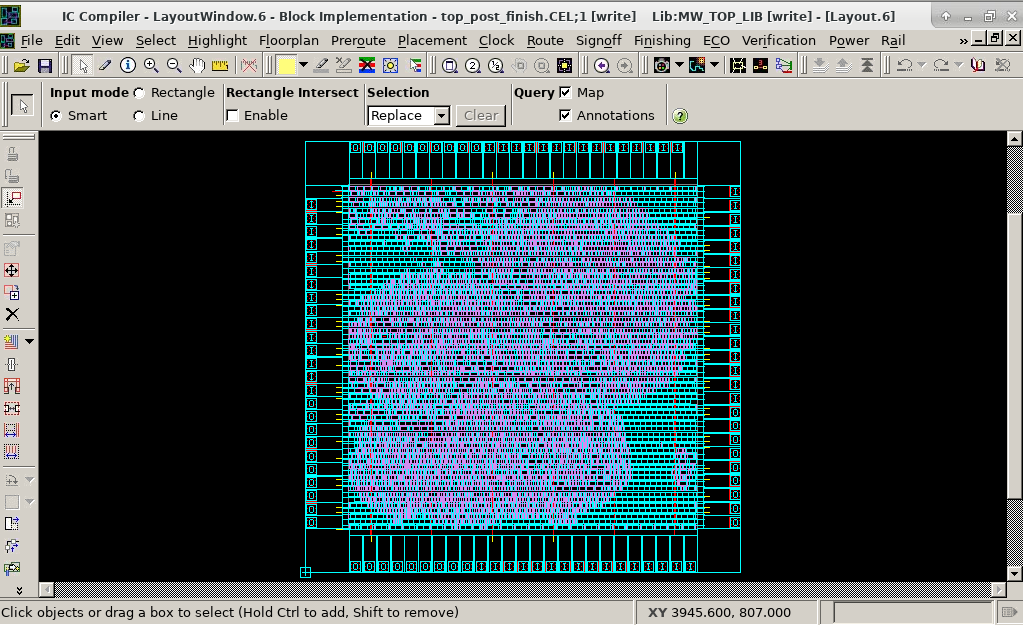
\includegraphics[scale=0.4]{./img/screenshot1}
\end{figure}

\begin{figure}[!htb]
\centering
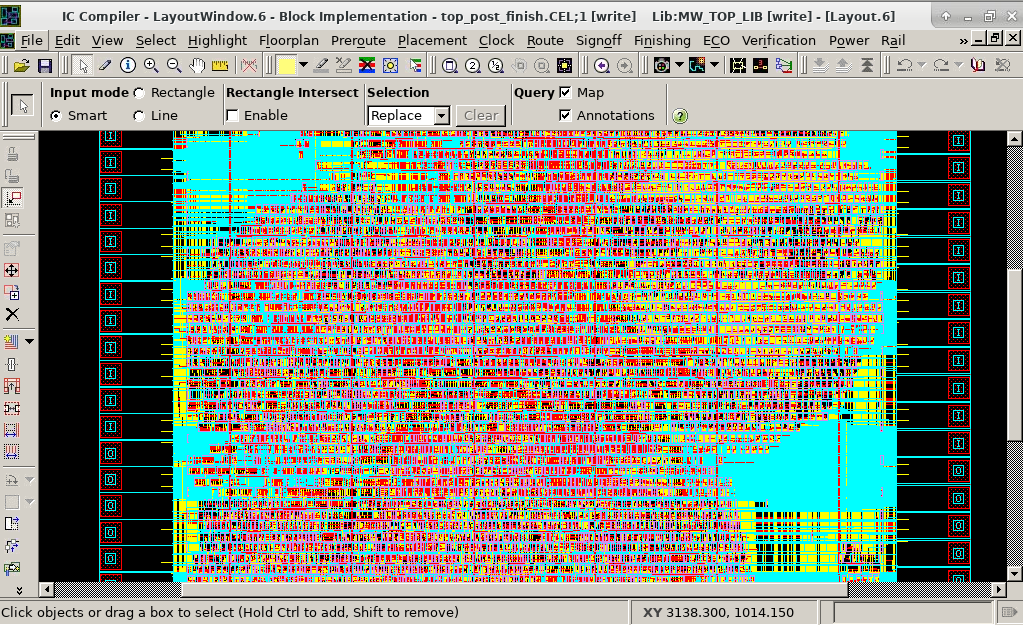
\includegraphics[scale=0.4]{./img/screenshot2}
\end{figure}

\begin{figure}[!htb]
\centering
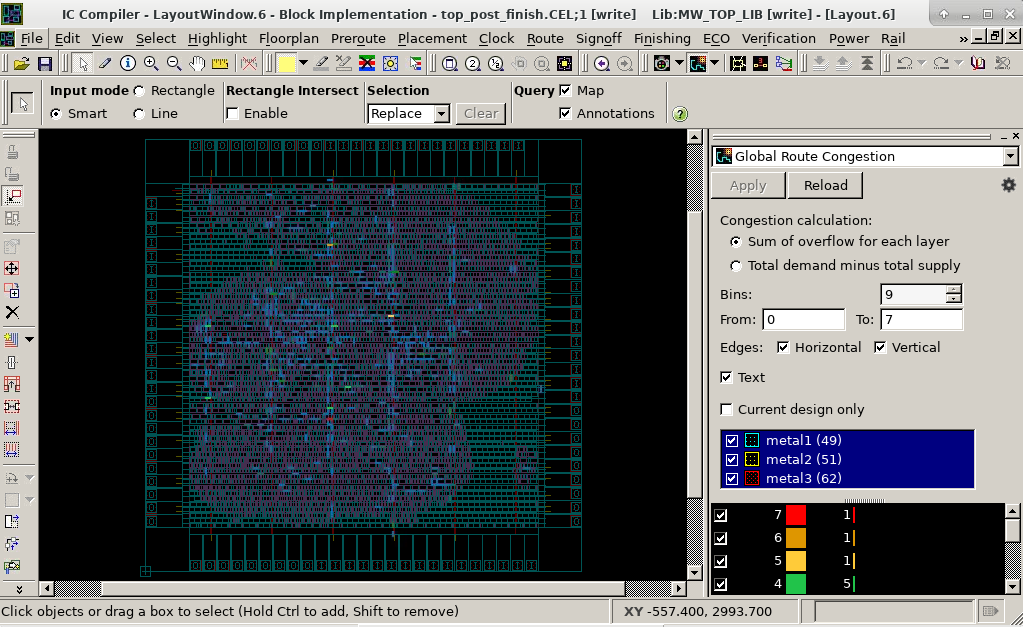
\includegraphics[scale=0.4]{./img/congestions}
\end{figure}

\end{document}